\documentclass{astroedu-lab}

\begin{document}

\pagestyle{plain}

\begin{problem}{\huge Лабораторная работа 3.6.1\\\\Спектральный анализ\\\\электрических сигналов\\\\Выполнил Жданов Елисей Б01-205}

\section{Цель работы:}

Изучить спектры сигналов различной формы и влияние параметров сигнала на вид соответствующих спектров

Проверить справедливость соотношений неопределённостей

Познакомиться с работой спектральных фильтров на примере RC-цепочки

\section{Оборудование:}

Экспериментальная установка состоит из генератора сигналов произвольной формы и цифрового USB-осциллографа, подключённого к персональному компьютеру

\section{Теоретическая справка}

Ряд Фурье и спектральный анализ. Согласно теореме Фурье, любая периодическая функция может быть представлена в виде ряда (конечного или бесконечного) гармонических функций с кратными частотами - pяда Фурье (см. п. 2.1. Введения к разделу). Одно из представлений ряда Фурье для функции с периодом $T$ имеет вид
$$
f(t)=\frac{A_0}{2}+\sum_{n=1}^{\infty} A_n \cos \left(2 \pi v_n t\right)+B_n \sin \left(2 \pi v_n t\right)
$$
циенты разложения в ряд Фурье. Коэффициенты находятся как
$$
A_n=\frac{2}{T} \int_0^T f(t) \cdot \cos \left(2 \pi v_n t\right) d t, \quad B_n=\frac{2}{T} \int_0^T f(t) \cdot \sin \left(2 \pi v_n t\right) d t .
$$

На практике зачастую удобнее использовать эквивалентную форму записи ряда Фурье в «представлении амплитуд и фаз»:
$$
f(t)=\frac{a_0}{2}+\sum_{n=1}^{\infty} a_n \cos \left(2 \pi v_n t+\varphi_n\right),
$$

где по известной тригонометрической формуле амплитуда гармоники равна $a_n=\sqrt{A_n^2+B_n^2}$, а фаза определяется соотношением $\operatorname{tg} \varphi_n=B_n / A_n$.

Отметим, что если функция $f$ чётная, то $B_n \equiv 0$ ( $\varphi_n \equiv 0$, разложение по косинусам), а если нечётная, то $A_n \equiv 0$ ( $\varphi_n \equiv \pi / 2$, разложение по синусам).

Совокупность всех частот $v_n$ и соответствующих им амплитуд $a_n$ (а также фаз $\varphi_n$ ) часто называют спектром функции $f(t)$. Если речь идёт об изменяющемся во времени напряжении, то говорят о спектре электрического сигнала.

Спектральный анализ электрических сигналов играет важную роль в технике. Особенно важен он для линейных систем, подчиняющихся принципу суперпозиции. Если известно, как некоторая система реагирует на гармонический сигнал, с помощью разложения Фурье можно определить, как система будет реагировать на произвольную функцию $f(t)$.

Заметим, что спектр периодической функции дискретен (число гармоник счётно). Если функция не периодическая (но ограниченная во времени, например, отдельный «импульс»), её можно представить как предел периодической функции с очень большим периодом $T \rightarrow \infty$. Тогда частотное расстояние между соседними гармониками $\delta v=1 / T$ стремится к нулю. Говорят, что спектр становится непрерывным. Разложение в ряд Фурье при этом переходит в интеграл Фурье (см. п. 2.2 Введения).

Операцию, при которой функции $f(t)$ ставится в соответствие её ряд (или интеграл) Фурье называют преобразованием Фурье. Это преобразование является взаимно-однозначным, а восстановление исходной функции по её спектру называется обратным преобразованием Фурье. Однако при спектральном анализе электрических сигналов, как правило, измеряются именно амплитуды $\left|a_n\right|$ (или интенсивности $\left|a_n\right|^2$ ) спектральных компонент, а информация об их фазах $\varphi_n$ теряется. Это приводит к тому, что пропадает взаимно-однозначное соответствие между сигналом и спектром, и весьма разные сигналы могут иметь один и тот же амплитудный спектр (пример: амплитудная и фазовая модуляции).

Соотношения неопределённостей. Между сигналом как функцией времени $f(t)$ и его спектром как функции частоты $a(v)$ имеется простая и универсальная взаимосвязь. А именно, если у сигнала $f(t)$ есть какое характерное время $\Delta t$ (например, период повторения, длительность импульса, время нарастания и т.п.), то в спектре $a(v)$ в том или ином виде будет наблюдаться характерный масштаб $\Delta v \sim 1 / \Delta t$ (расстояния между пиками, ширина спектра, ширина пиков и т.п.).
Соотношения вида
$\Delta v \cdot \Delta t \sim 1$

принято называть соотношениями неопределённостей. Конкретный вид соотношения неопределённостей зависит от обстоятельств, в которых оно применяется.

Например, если $\Delta t=\tau$ - характерная длительность импульса, то характерная ширина спектра по порядку величины будет равна $\Delta v \sim 1 / \tau$. Здесь единица в правой части (4) - это единица именно по порядку величины. Конкретное числовое значение зависит, во-первых, от детальной формы сигнала, и, во-вторых, от того, что именно мы называем «характерным» временем и что - «шириной» спектра.

Другой пример, для любого сигнала с периодом $T$ в спектре обязательно будут наблюдаться гармоники на расстоянии $\delta v=1 / T$ друг от друга. В данном случае соотношение является точным и от формы сигнала не зависит.

Методы спектрального анализа. Современные методы спектрального анализа электрических сигналов можно разделить на два типа: цифровые (математические) и аналоговые (физические).

Простейшим физическим анализатором частот является высокодобротный колебательный контур ( $R L C$-цепочка). Такой контур, как известно, хорошо откликается на частоты, близкие к его резонансной, и почти не реагирует на частоты, находящиеся за пределами его узкой (т.к. контур высокодобротный) амплитудно-частотной характеристики. Подстраивая параметры контура и изменяя его резонансную частоту, можно «просканировать» весь частотный спектр поступающего на него сигнала. В современной лаборатории спектральные приборы, основанные на физических методах (как правило, довольно дорогостоящие), применяются для анализа высоких частот (сотни мегагерц и более).

Если же частота исследуемого сигнала не слишком велика (заведомо меньше тактовой частоты процессоров), современная цифровая техника позволяет проводить частотный анализ сигналов в реальном времени непосредственно по математическим формулам (2). Входящий сигнал при этом оцифровывается (дискретизуется) и, с помощью так называемого алгоритма «быстрого преобразования Фурье», осуществляется вычисление частот и амплитуд его гармоник.

Цифровой спектральный анализ имеет две отличительные особенности, о которых стоит упомянуть.

Во-первых, при цифровом анализе возникает частота дискретизадаваемого на входной канал анализатора. Ясно, что дискретизация не позвовблизи неё. Поэтому надёжно получать спектр можно лишь на достаточно низких частотах $v \ll v_{\text {дискр }}$, когда влияние дискретности минимально (точнее, как следует из теоремы Котельникова, необходимо выполнение условия $v<v_{\text {дискр }} / 2$ ). Внутренняя частота дискретизации осциллографов обычно велика (типичное значение - 1 ГГц), однако для преобразования Фурье в целях оптимизации скорости работы она может существенно урезаться. В настройках цифровых осциллографов часто используется параметр «количество точек» на интервал времени. Например, если сигнал записывался в течение 1 c, то при стандартных для многих осциллографов 4096 точках дискретизации, спектр будет заведомо ограничен лишь частотой $~ 2$ кГц!

Во-вторых, интервал времени $\Delta t$, в течение которого регистрируется сигнал, всегда ограничен. Для анализа сигнала вырезается его участок - «окно» $t \in\left[t_0 ; t_0+\Delta t\right]$. Такое преобразование Фурье часто называют «оконным». Изза ограниченности размеров «окна» неизбежно возникают дополнительные искажения спектра (их можно назвать «краевыми эффектами»). Чтобы компенсировать эти искажения, значениям регистрируемой функции в пределах «окна» придают разный вес. В таком случае говорят об «оконной» (или «весовой») функции преобразования Фурье. На практике применяются различные оконные функции, каждая из которых обладает своими достоинствами и недостатками (одни уменьшают шумы, другие уменьшают ширину пиков и погрешность частоты, третьи погрешность измерения амплитуд и т.д.). В нашей работе важно аккуратное измерения амплитуд, для чего лучше всего подходят окна «с плоской вершиной» (flat top) и, в меньше степени, Блэкмана (Blackman). Для более точного измерения частот предпочтительнее окна Ханна (Hann) и Хэмминга (Hamming).

\section{Измерения, Обработка}

1) По техническому описанию ознакомимся с устройством панелей приборов: генератора сигналов произвольной формы и цифрового осциллографа / компьютерной программы, используемой для отображения сигналов с осциллографа. Изучим расположение основных кнопок и ручек настройки.

2) Подключим один из выходов генератора к одному из каналов осцилло-графа и включим приборы в сеть.

\subsection{А. Исследование спектра периодической последовательности прямоугольных импульсов и проверка соотношений неопределённостей}

\begin{figure}[!h]
	\centering
	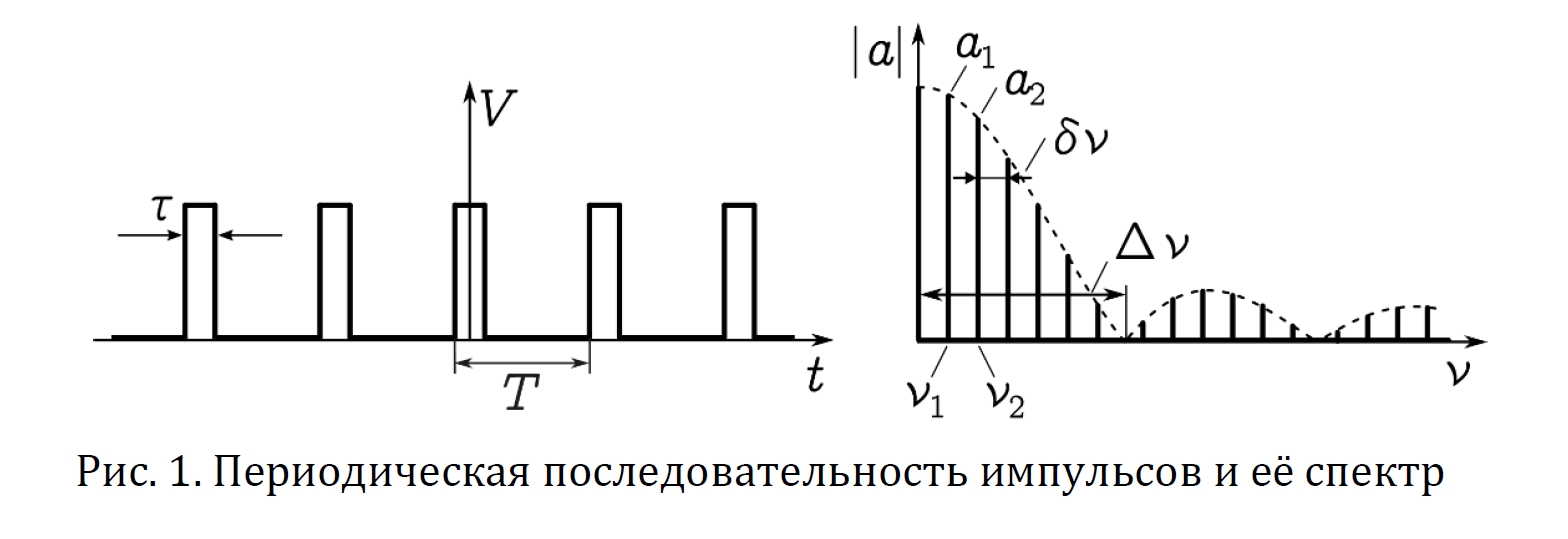
\includegraphics[width=0.85\textwidth]{im/1.png}
	\label{fig:boiler}
\end{figure}

3-4) Настроим генерацию прямоугольных импульсов с параметрами частоты повторения $v_{\text {повт }}=1$ кГц (период $\left.T=1 / v_{\text {повт }}=1 \text{ мc}\right)$, и длительность импульса $\tau=$ $T / 20=50$ мкс. Получим устойчивую картину сигнала на экране осциллографа.

5) Получим на его экране спектр (преобразование Фурье) сигнала.

6) Изменяя на генераторе параметры сигнала, наблюдайте, как изменяется спектр. Запишите в лабораторном журнале, что происходит со спектром:

а) при изменении $v_{\text {повт }}$ при фиксированном $\tau$

Экстремумы огибающей спектра не двигаются по горизонтали, максимумы меняют амплитуду, а голичество гармоник в одной секции спектра уменьшается при увеличении частоты.

б) при изменении $\tau$ при фиксированном $v_{\text {повт }}$.

При увеличении $\tau$ количество гармоник в одной секции уменьшается и наоборот. При это экстремумы сжимаются к нулевой частоте, что аналогично масштабированию спектра.

Сохраните или сфотографируйте несколько (3-4) спектров с различными параметрами (при фиксированных масштабах частот по горизонтали кГц/дел и амплитуд по вертикали).

Изображения приложите к отчёту и прокомментируйте их различия.

7) Ознакомьтесь с методикой измерения параметров спектра (см. техническое описание осциллографа, п. III). При некоторых фиксированных параметрах $v_{\text {повт }}$ и $\tau$ (например, заданных в п. 3) измерьте амплитуды $a_n$ и частоты $v_n$ нескольких (6-8) спектральных компонент (гармоник). Сравните значения с рассчитанными теоретически (см. Пример 3 Введения к разделу VI):
$$
v_n=\frac{n}{T}, \quad\left|a_n\right|=\frac{\left|\sin \frac{\pi n \tau}{T}\right|}{\pi n}=\frac{\tau}{T} \frac{\left|\sin \pi v_n \tau\right|}{\pi v_n \tau} .
$$

Поскольку единицы измерения амплитуд гармоник произвольны, следует сравнивать их относительные величины, например $\left|a_n / a_1\right|$. Результаты занесите в таблицу:
\begin{center}
\begin{tabular}{|c|c|c|c|c|c|c|}
\hline$n$ & 1 & 2 & 3 & 4 & 5 & 6 \\
\hline$v_n^{\text {эксп }}$, кГц & 1.106 & 2.065 & 3.024 & 4.143 & 5.262 & 6.221 \\
\hline$v_n^{\text {тeop }}$, кГц & 1 & 2 & 3 & 4 & 5 & 6 \\
\hline$\left|a_n\right|^{\text {эксп }}$, дБ & -8.782 & -8.93 & -9.225 & -9.52 & -10.11 & -10.7 \\
\hline$\left|a_n / a_1\right|^{\text {эксп }}$ & 1 & 0.98 & 0.95 & 0.92 & 0.86 & 0.80 \\
\hline$\left|a_n / a_1\right|^{\text {reop }}$ & 1 & 0.99 & 0.97 & 0.94 & 0.90 & 0.86 \\
\hline
\end{tabular}
\end{center}

%!!!!!!!!!!!!!!!!!!!!!!!!!!!!!!!!!!!!!!!!!!!
%Далее будет excel
%!!!!!!!!!!!!!!!!!!!!!!!!!!!!!!!!!!!!!!!!!!!

8) Зафиксируйте период повторения $T$ прямоугольного сигнала (например, $T=1$ мс, $v_{\text {повт }}=1$ кГц). Изменяя длительность импульса $\tau$ в диапазоне от $\tau=T / 50$ до $\tau=T / 5$, измерьте полную ширину спектра сигнала $\Delta v-$ от центра спектра $(v=0)$ до гармоники с нулевой амплитудой $a_n \approx 0$.

9) Зафиксируйте длительность импульса прямоугольного сигнала (например, $\tau=100$ мкс). Изменяя период повторения $T$ в диапазоне от $2 \tau$ до $50 \tau$ измерьте расстояния $\delta v=v_{n+1}-v_n$ между соседними гармониками спектра. Если спектральные компоненты окажутся расположены слишком близко друг к другу, измерьте расстояние между $(n+m)$-й и $m$-й гармониками (для некоторых целых $n$ и $m$ ) найдите $\delta v=\left(v_{n+m}-v_n\right) / m$.

10) Постройте графики зависимостей $\Delta v(1 / \tau)$ и $\delta v(1 / T)$. Проведите наилучшие прямые и определите их наклон. Убедитесь в справедливости соотношений неопределённости (см. п. 2.3. Введения). Оцените погрешности.

\subsection{Б. Наблюдение спектра периодической последовательности цугов}

\begin{figure}[!h]
	\centering
	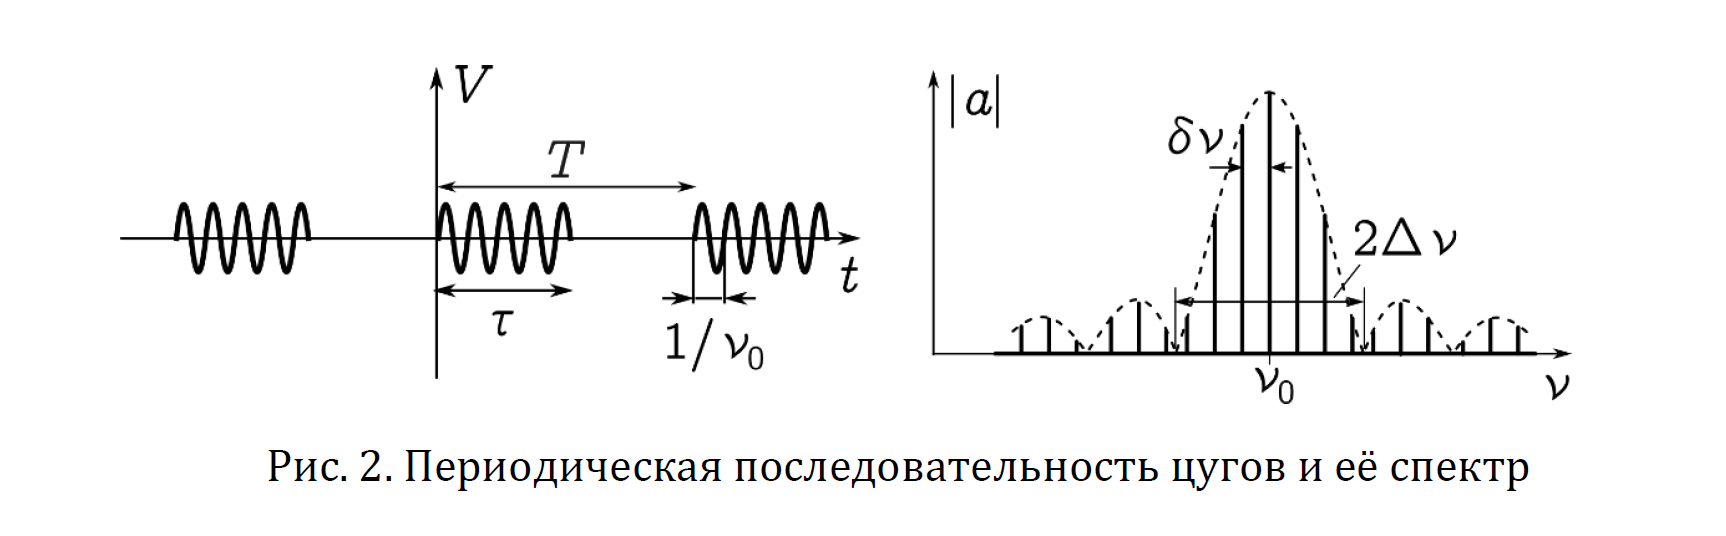
\includegraphics[width=1\textwidth]{im/2.png}
	\label{fig:boiler}
\end{figure}

11) Следуя техническому описанию генератора (п. Б), установите на режим подачи периодических импульсов синусоидальной формы («цугов»). Рекомендуемые параметры: частота несущей $v_0=50$ кГц, период повторения
$T=1$ мс ( $v_{\text {повт }}=1$ кГц), число периодов синусоиды в одном импульсе $N=5$ (что соответствует длительности импульса $\tau=N / v_0=100$ мкс). Получите на экране осциллографа устойчивую картину сигнала.

12) Получите на экране осциллографа спектр сигнала. Центр картины установите на частоту $v_0$. Масштаб по горизонтали (кГц/дел) подберите так, чтобы спектр помещался на экране.

13) Изменяя параметры сигнала $v_0 = 50 \text{ кГц}, T$ и $N$ наблюдайте, как изменяется вид спектра. Сравните наблюдаемые спектры со спектрами прямоугольных импульсов. Сохраните или сфотографируйте несколько (3-4) изображений спектров, подтверждающих результаты наблюдений. Изображения приложите к отчёту и прокомментируйте их.

Меняем частоту - растягиваем спектр вдоль оси координат.

Меняем N - меняем количество частот в сегменте спектра.

Изменение T - аналогично N, только без сдвига мексимумов

14) При параметрах сигнала, соответствующих сохранённым в предыдущем пункте изображениям, измерьте положение центра спектра, его ширину $\Delta v$ и расстояние между гармониками $\delta v$. Убедитесь в справедливости теоремы смещения (см. п. 3 Введения) и соотношений неопределённостей.

При частотах $\nu$ от 1 до 10 кГц $\delta \nu$ совпадает с частотой, а значит соотношение неопределенностей выполняется.

\subsection{Г. Исследование спектра амплитудно-модулированного сигнала}

\begin{figure}[!h]
	\centering
	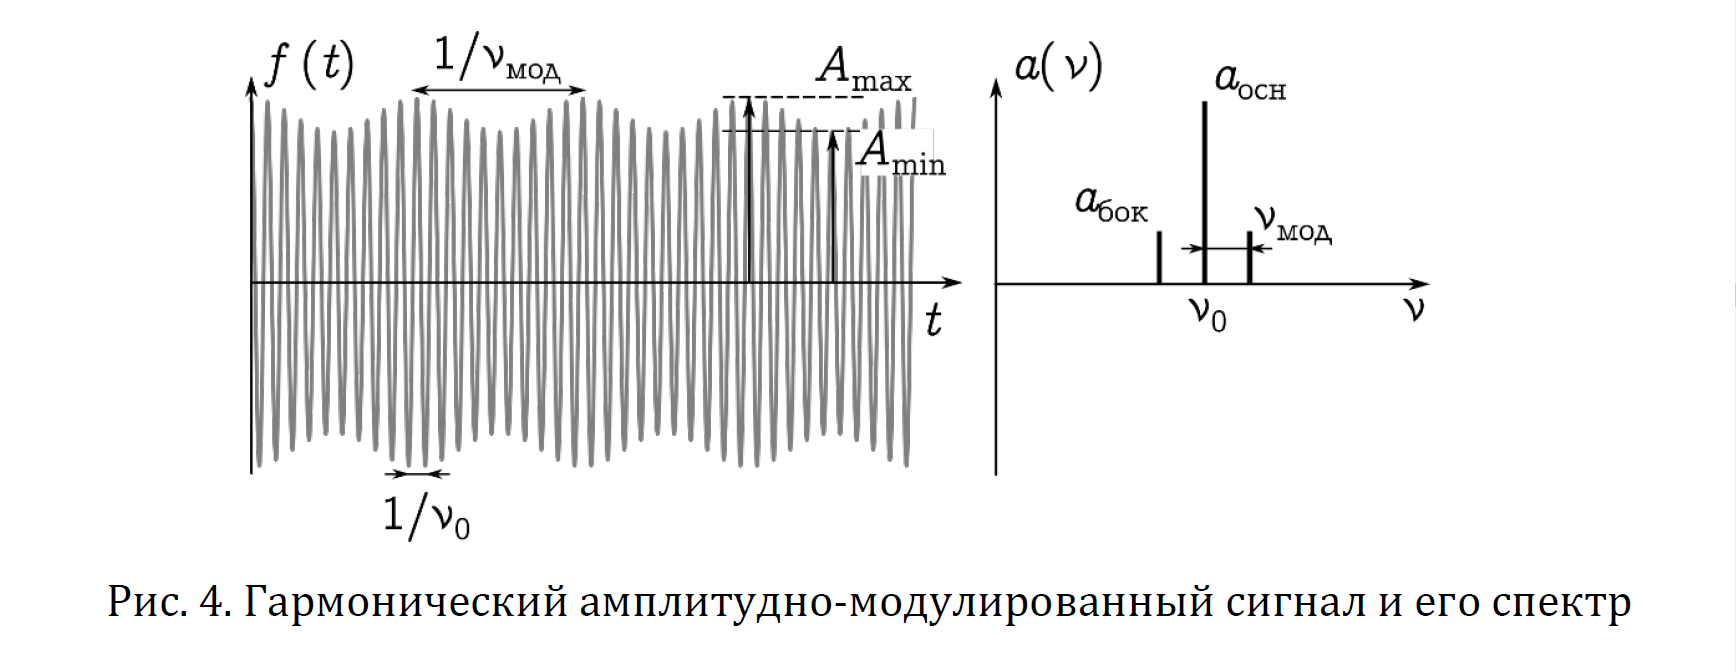
\includegraphics[width=1\textwidth]{im/4.png}
	\label{fig:boiler}
\end{figure}

19) Установили сигнал, сделали фотографию

20) Действительно 1.474 В и 0.475 В - максимальная и минимальная амплитуды. Соотношение $\frac{A_{max} - A_{min}}{A_{max} + A_{min}} \approx 0.5$ 

21) При изменении частоты модуляции вверх, гармоники вместе сдвигаются вправо(в область высоких частот).

При изменении несущей частоты вдали от 60 кГц происходит сдвиг картинки по оси абсцисс. Около же этой частоты, частоты модуляции сдвигаются относительно несущей частоты.

23) Как видим, m/2 совпадает с отношением амплитуд сигналов. Теория сходится с практикой.

\subsection{Д. *Наблюдение спектра сигнала, модулированного по фазе}

24) Развертка сигнала немного дрожит по фазам

25) Фактически, при изменении частот, изменение спектра тождественно изменениям в предыдущем пункте. Однако, когда мы увеличиваем максимальное отклонение глубины модуляции фазы более 90$^\circ$, то получаем спектр различных частот, а не только 2 модуляционные.

\subsection{Е. Изучение фильтрации сигналов}

\begin{figure}[!h]
	\centering
	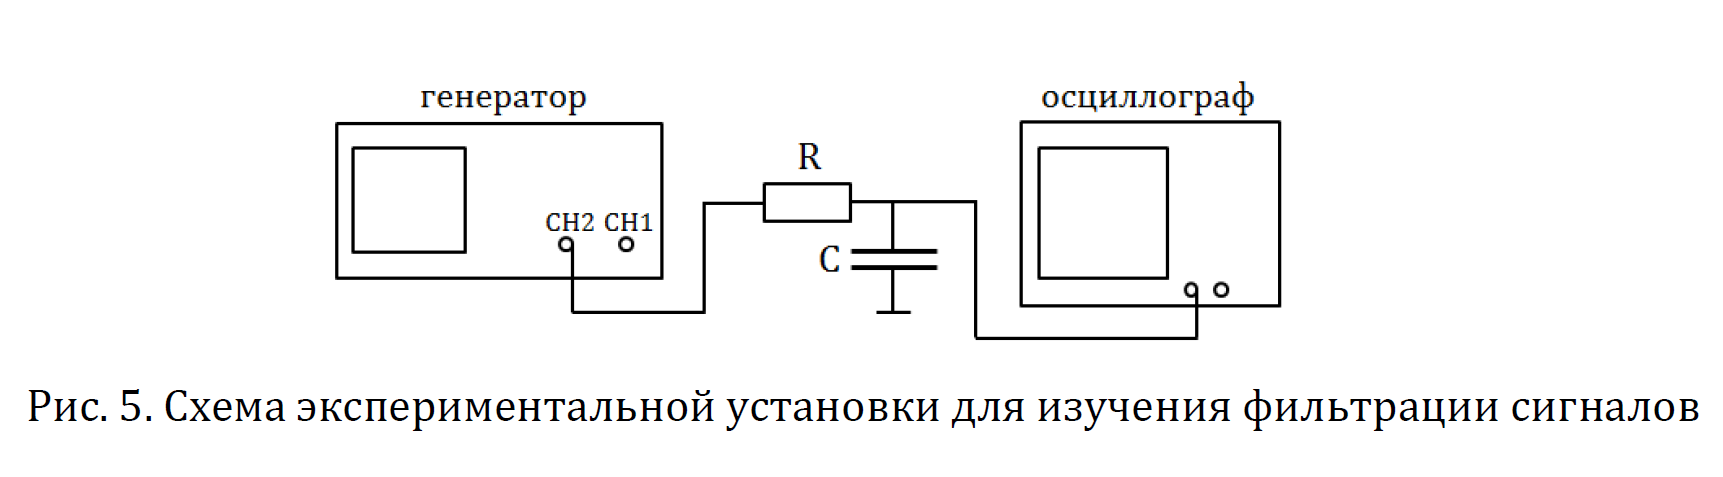
\includegraphics[width=1\textwidth]{im/5.png}
	\label{fig:boiler}
\end{figure}

\begin{center}
\begin{tabular}{|c|c|c|c|}
\hline 
\multicolumn{2}{|c|}{$h_\text{ман}$, мм} & $\sigma, \frac{\text{мН}}{\text{К}}$ & T, $^\circ$C \\
\hline
188.0 & 188.0 & $(64.5 \pm 3.9)$ & 22\\
187.0 & 187.0 & $(64.0 \pm 3.9)$ & 30\\
185.5 & 186.0 & $(63.3 \pm 3.9)$ & 35\\
184.0 & 184.5 & $(62.5 \pm 3.9)$ & 40\\
182.5 & 183.0 & $(61.7 \pm 3.9)$ & 45\\
181.0 & 181.0 & $(60.8 \pm 3.8)$ & 50\\
179.0 & 179.5 & $(59.9 \pm 3.8)$ & 55\\
177.5 & 177.5 & $(59.0 \pm 3.8)$ & 60\\
\hline
\end{tabular}
\end{center}


Найдем угловые коэффициенты прямых для каждой установки по МНК.

\[
	a = \frac{<x_i y_i> - < x > < y_i >}{< x_i^2> - < x_i >^2}
\]

\[
	b = < \nu_i > - a < N_i >
\]

Также рассчитаем их погрешности

\begin{equation}
	S_a^2 = \frac{< x_i^2>}{< x_i^2 > - < x_i >^2} \cdot \frac{<  b_i - b > ^2}{n - 2}
\end{equation}


\begin{center}
	\Large $q(T)$
\end{center}

\section{Вывод}


\section{Ресурсы}

Расчет по МНК: метод-наименьших-квадратов.рф


\end{problem}
\end{document}